\chapter{\glsentrylong{JPEG} (\glsentryshort{JPEG})}

\section{\glsentryshort{ITU} standard}
\begin{itemize}
\item Supported by all Web browsers, and most image viewers, define
  how to compress raster images \cite{ccitt.t81,wikipedia_ITU}.
\item Developed by the \gls{JPEG} (\href{https://www.itu.int}{ITU}),
  in 1992 \cite{wikipedia_JPEG}.
\end{itemize}

\begin{figure}[H]
  \vspace{-2ex}
  \centering
  \href{https://en.wikipedia.org/wiki/Magnetic_resonance_imaging_of_the_brain#/media/File:MRI_of_Human_Brain.jpg}{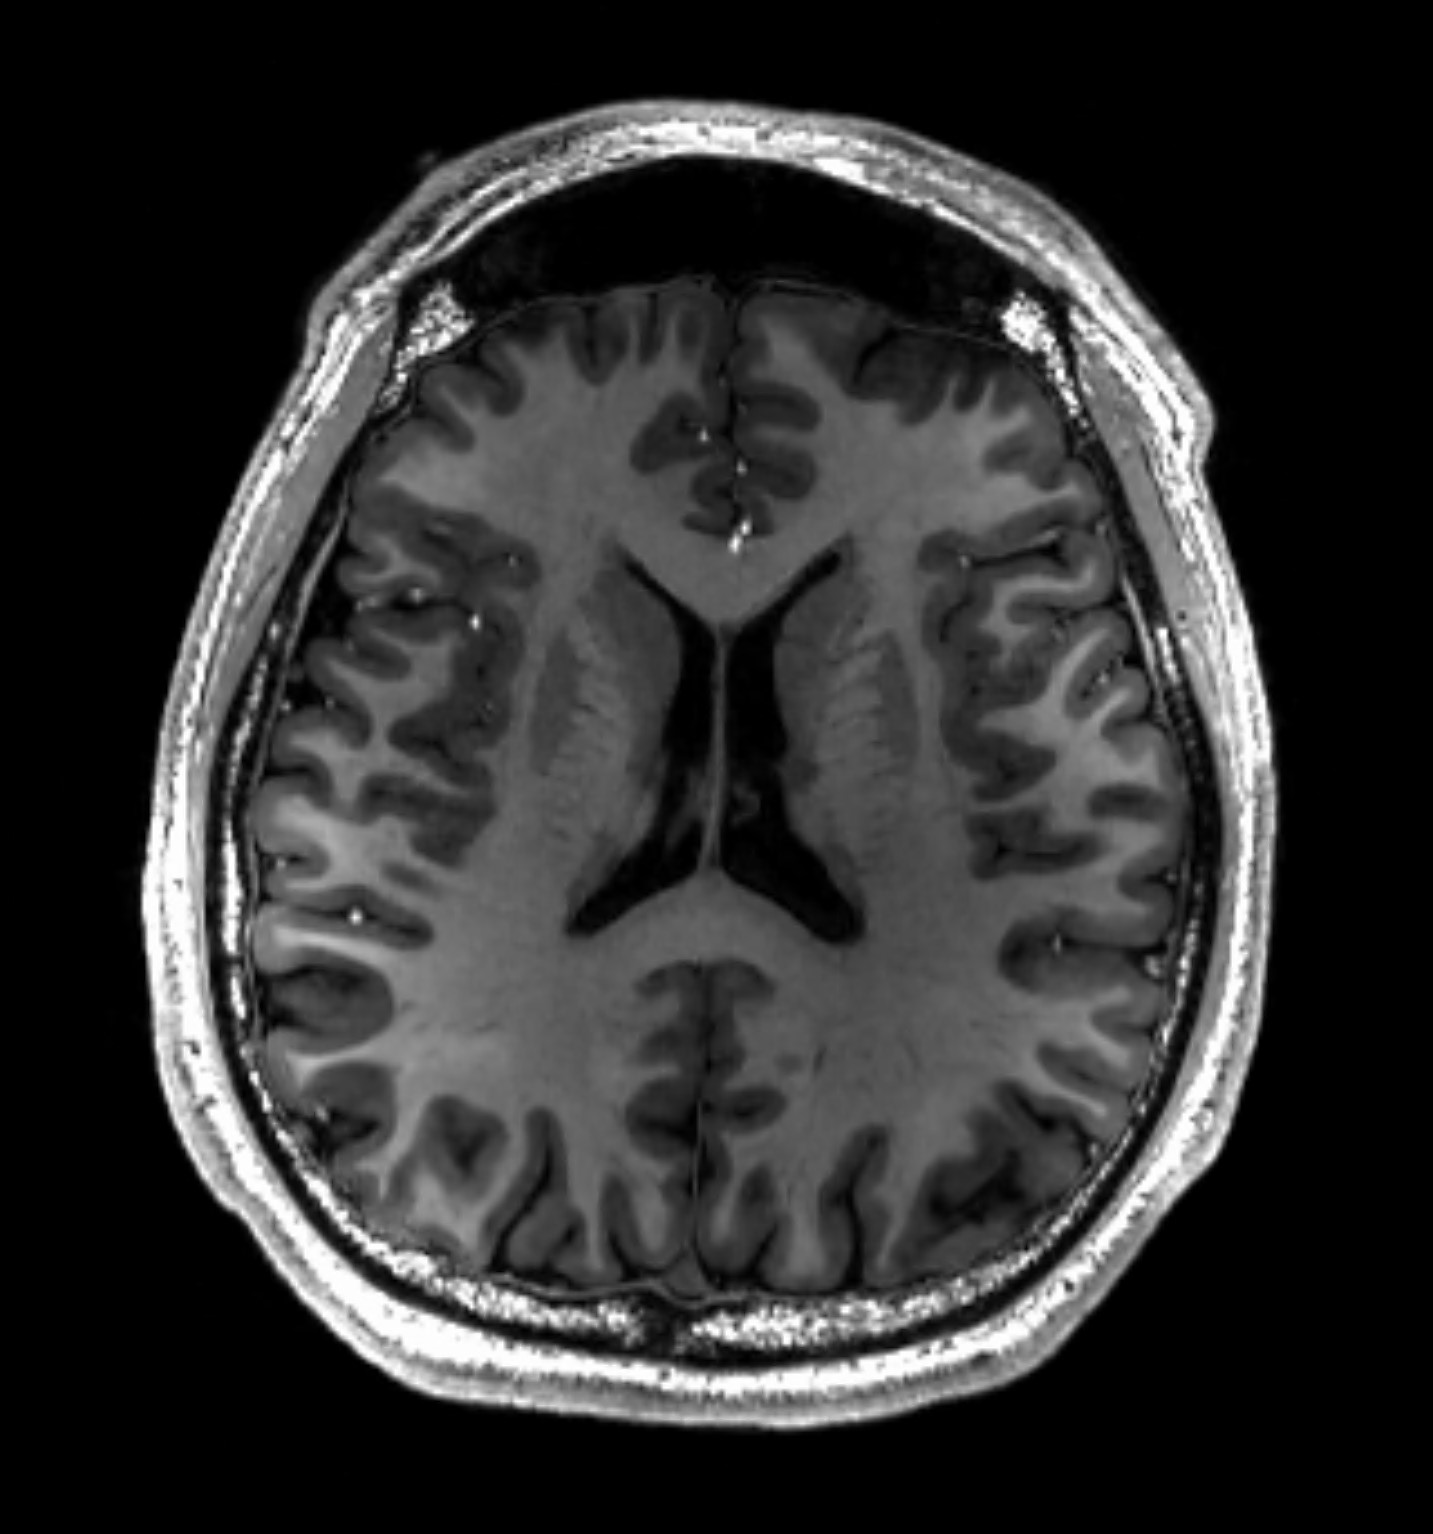
\includegraphics[width=4.0cm]{MRI_of_Human_Brain}}
  \caption{A \gls{JPEG} version of a medical image.}
  \label{fig:JPEG_example}
\end{figure}

\section{Lossy compression of color natural images}
\begin{itemize}
\item Designed for achieve high compression ratios, but at the expense of reducing quality.
  \item Raster images with up to $(2^{16}-1)\times (2^{16}-1)$ pixels.
  \item Pixels must be gray-scale or \gls{RGB}, 8 bits/channel.
\end{itemize}

\begin{figure}[H]
  \vspace{-0ex}
  \centering
  \href{https://www.thewebmaster.com/jpeg-definitive-guide/}{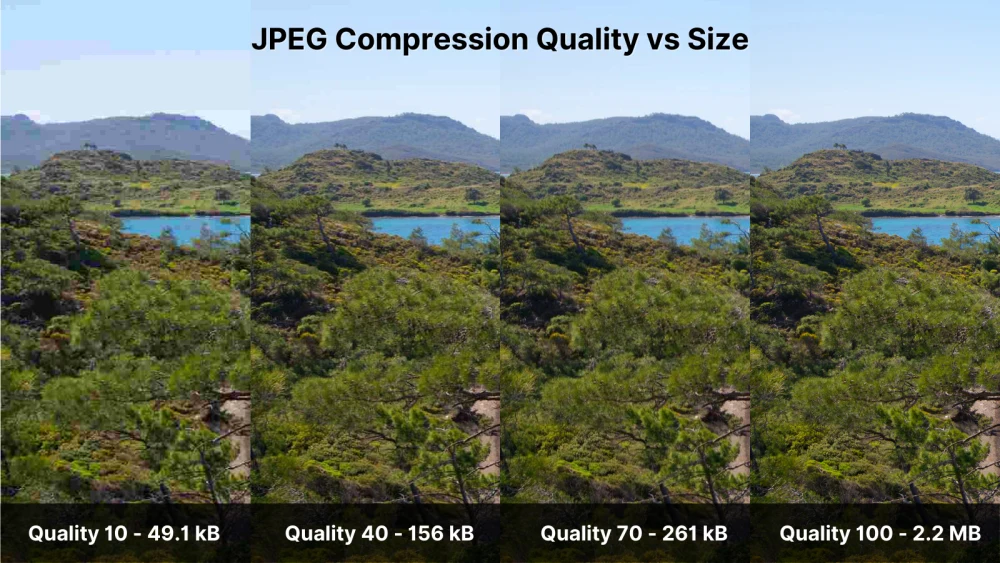
\includegraphics[height=\textheight]{JPEG_Quality_vs_Size}}
  \caption{The lossy effect in a \gls{JPEG} image.}
  \label{fig:JPEG_lossy}
\end{figure}

\section{Algorithm}
\begin{enumerate}
\item Convert from the \gls{RGB} color space to the \gls{YCbCr} color
  space. Only if the input image is in color.
\item Subsample the chrominance (Cr and Cb channels). /* Lossy step */
\item Divide each channel in blocks of size 8x8. \popup{The rest of
    steps work by blocks}{This makes it possible to work at the block
    level regardless of the image size.}.
\item Transform each block using the \gls{DCT}.
\item Quantize the \gls{DCT} coefficients. /* Lossy step */
\item Entropy encode the quantized coefficients.
\end{enumerate}

\begin{figure}%[H]
  %\vspace{-2ex}
  \centering
  \href{https://link.springer.com/article/10.1007/s40799-019-00358-4}{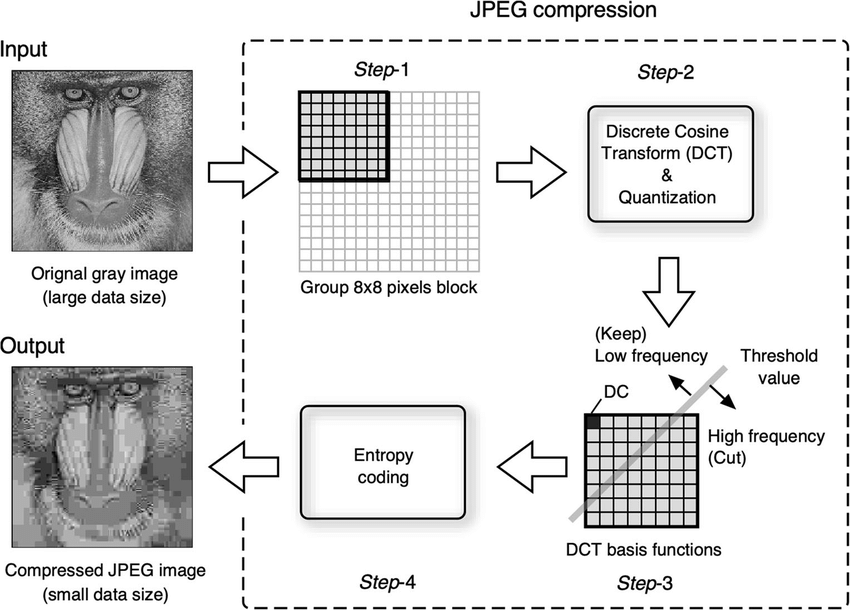
\includegraphics[height=1.0\textheight]{JPEG}}
  \caption{The \gls{JPEG} compression scheme.}
  \label{fig:JPEG_compressor}
\end{figure}

\section{Blocking}
  %\vspace{-4ex}
\begin{figure}[H]
  \centering
  \href{https://thesai.org/Publications/ViewPaper?Volume=6&Issue=4&Code=ijacsa&SerialNo=16}{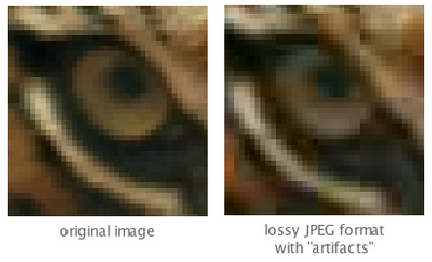
\includegraphics[height=0.8\textheight]{JPEG_blocking}}
  \caption{\gls{JPEG} blocking artifacts.}
  \label{fig:JPEG_blocking}
\end{figure}

\section{Progressive rendering}
\begin{itemize}
\item Optional. Blocks are reconstructed coefficient-by-coefficient following the zig-zag ordering.
\item During a progressive visualization, blocks display higher
  spatial frequencies, progressively, in each rendering.
\end{itemize}

\begin{figure}[H]
  \vspace{-2ex}
  \centering
  \href{https://es.m.wikipedia.org/wiki/Archivo:Zigzag_scanning.jpg}{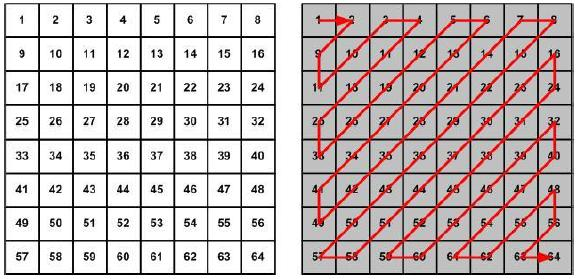
\includegraphics[width=8cm]{Zigzag_scanning}}
  \caption{Progressive visualization in \gls{JPEG}.}
  \label{fig:JPEG_progressive}
\end{figure}

\section{Metadata}
\begin{itemize}
\item \gls{JPEG} images can store metadata as
  \href{https://en.wikipedia.org/wiki/Exif}{\gls{Exif}} data (see the
  \href{https://gitlab.com/TNThieding/exif/-/blob/master/docs/api_reference.rst?ref_type=heads}{Exif
    implementation}). In the Table~\ref{tab:JPEG_metadata} there are
  some of the supported fields:
  \begin{table}[!h]
    \vspace{2ex}
    \begin{center}
      \begin{tabular}{l|l}
        Keyword & Meaning\\
        \hline
        ImageWidth & Width of the image in pixels \\
        ImageLength & Height of the image in pixels \\
        BitsPerSample&  Number of bits per color \\
        Make & Manufacturer of the camera or scanner \\
        Model & Model of the camera or scanner \\
        Software & Software used to process the image \\
        Orientation & Of the camera when the image was taken \\
        DateTimeOriginal & Date and time the image was originally captured \\
        ExposureTime & shutter speed \\
        FNumber & Lens aperture setting \\
        FocalLength & Focal length of the lens \\
        UserComment & User's comments about the image
      \end{tabular}
    \end{center}
    \caption{Metadata in a JPEG image.}
    \label{tab:JPEG_metadata}
  \end{table}
\end{itemize}

\section*{}
\begin{itemize}
\item
  \href{https://github.com/vicente-gonzalez-ruiz/medical_imaging/blob/main/notebooks/JPEG_add_metadata.ipynb}{Here}
  there is an example that shows and modifies the metadata in a JPEG
  image.
\end{itemize}
